\documentclass[11pt]{article}
\usepackage{times}
\usepackage{comment} % enables the use of multi-line comments (\ifx \fi)
\usepackage{fullpage} % changes the margin
\usepackage{graphicx}
\usepackage{subcaption}

\begin{document}
%Header-Make sure you update this information!!!!
\noindent
\large\textbf{Summary of Age-Oxygen Current Results} \hfill \textbf{Jordan Thomas} \\
05/10/2017 \\

\section*{Aim:}

Examine if the observed change in oxygen over the observational period is
consistent with the ventilation changes documented by Waugh et al., 2013.

Use the GFDL ESM2Mc to establish the relationship between ideal age and oxygen
in the Southern Ocean. Using the age changes found in Waugh et al., 2013,
determine if the observed change in oxygen is consistent with the changes in
circulation. Expectation that in SAMW where the age decreases, oxygen
concentration will increase. In CDW where age increases, oxygen concentration
will decrease.

% \section*{Methods:}
% Calculated the change of both dissolved oxygen and apparent oxygen utilization
% (AOU) for each repeat hydrography transect in the Southern Ocean. Following
% figure shows the percent change per decade for both oxygen and AOU for two
% watermasses: Subantarctic Mode Water (SAMW) and Circumpolar Deep Water (CDW).
% SAMW is defined as the water between latitudes 20S and 50S which lies between
% isopycnal surfaces 26.6 and 27.0. AABW is defined at the water South of 50S that
% lies between isopycnal surfaces 27.2 and 27.7.
%
% Apparent Oxygen Utilization is defined as the following:
% $$ AOU=O_2^{sat}−O_2 $$
% where $O_2$ is the measured dissolved oxygen and $O_2^{sat}$ is the calculated
% oxygen saturation. The oxygen saturation is calculated from the measured
% salinity and potential temperature following the empirical formulation
% described in Weiss, 1970.


\section*{Results - Model Age-Oxygen Relationship:}

\begin{enumerate}

\item Quantified model relationship between ideal age and oxygen/AOU for SAMW region.

\begin{figure*}[h!]
    \centering
    \begin{subfigure}[t]{0.5\textwidth}
        \centering
        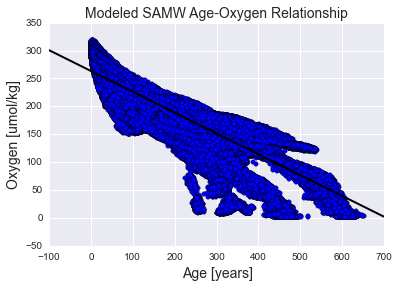
\includegraphics[height=2.25in]{modeled_samw_age_o2.png}
    \end{subfigure}%
    ~
    \begin{subfigure}[t]{0.5\textwidth}
        \centering
        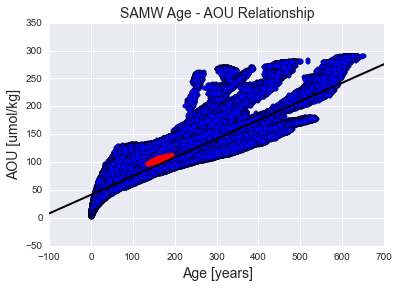
\includegraphics[height=2.25in]{modeled_samw_age_aou.png}
    \end{subfigure}
    \caption{Relationship between ideal age and oxygen (left) and apparent oxygen
    utilization (right) for SAMW region in GFDL ESM2Mc control simulation.}
\end{figure*}

\item Quantified the change in oxygen and AOU in SAMW region for each ship track.
\begin{itemize}
  \item Found negative trend in SAMW oxygen (~3\% per decade), except on track
  P16 which was slightly positive.
  \item Found positive trend in SAMW AOU (~10\% per decade).
  \item Very little change in CDW oxygen or AOU (not shown).
\end{itemize}

\textbf{This is the opposite response than suggested given the above relationship
between age and oxygen and the documented changes in SAMW age.}

\begin{figure*}[t!]
    \centering
    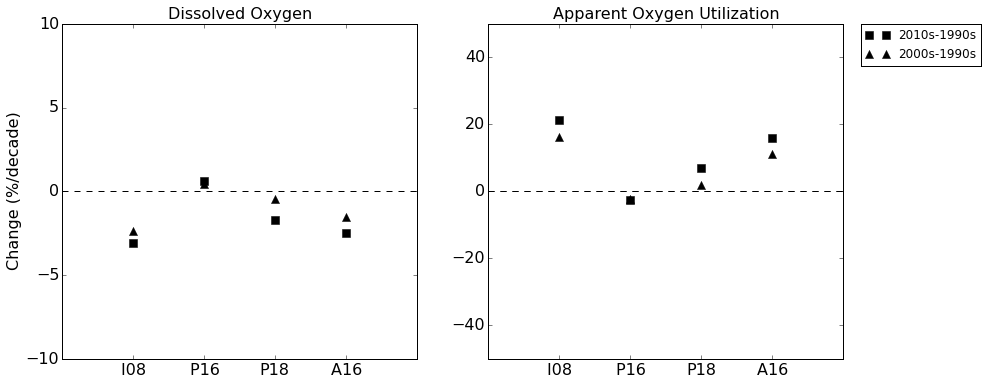
\includegraphics[height=2.25in]{change_oxygen.png}
    \caption{Percent change oxygen (left) and AOU (right) for entire time series
    (squares) and first decade (triangles).}
\end{figure*}

\textbf{}


\item Next aim to understand why we see a decrease in oxygen (increase in AOU) when the
opposite is expected given the documented changes in ventilation. Look at oxygen
utilization rates, other literature, ect.
\end{enumerate}

\clearpage


\section*{Supplemental Figures:}
\begin{figure*}[h!]
    \centering
    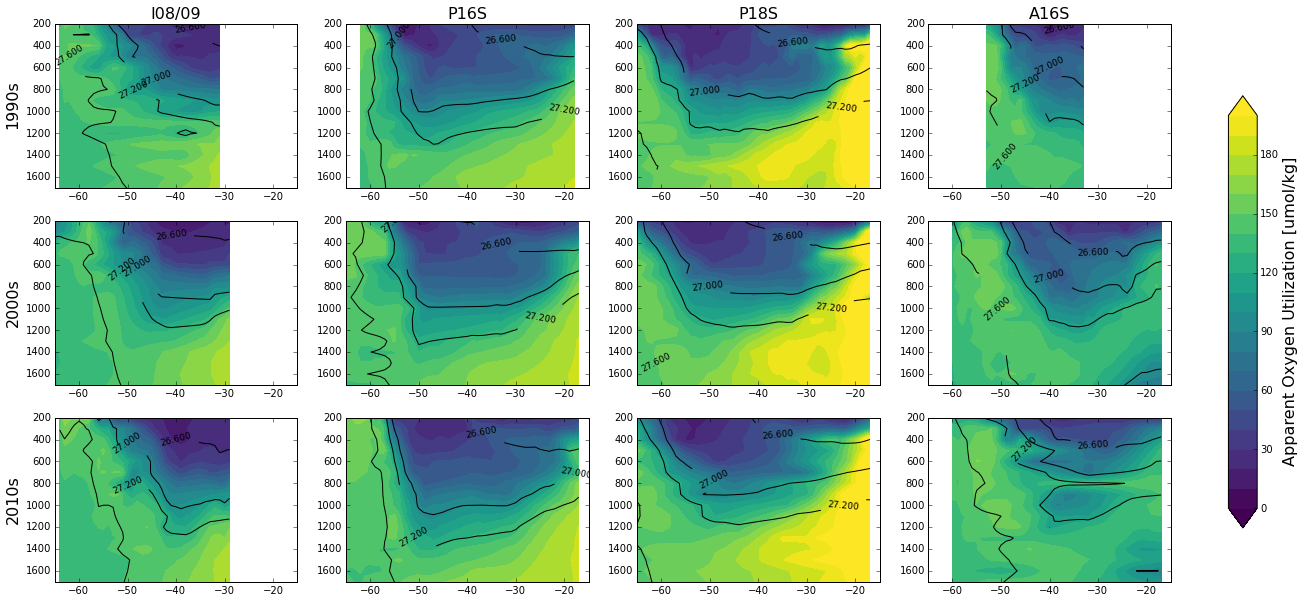
\includegraphics[height=3in]{AOU_clim.png}
    \caption{AOU spatial patterns for each transect and each sample year.}
\end{figure*}

\begin{figure*}[h!]
    \centering
    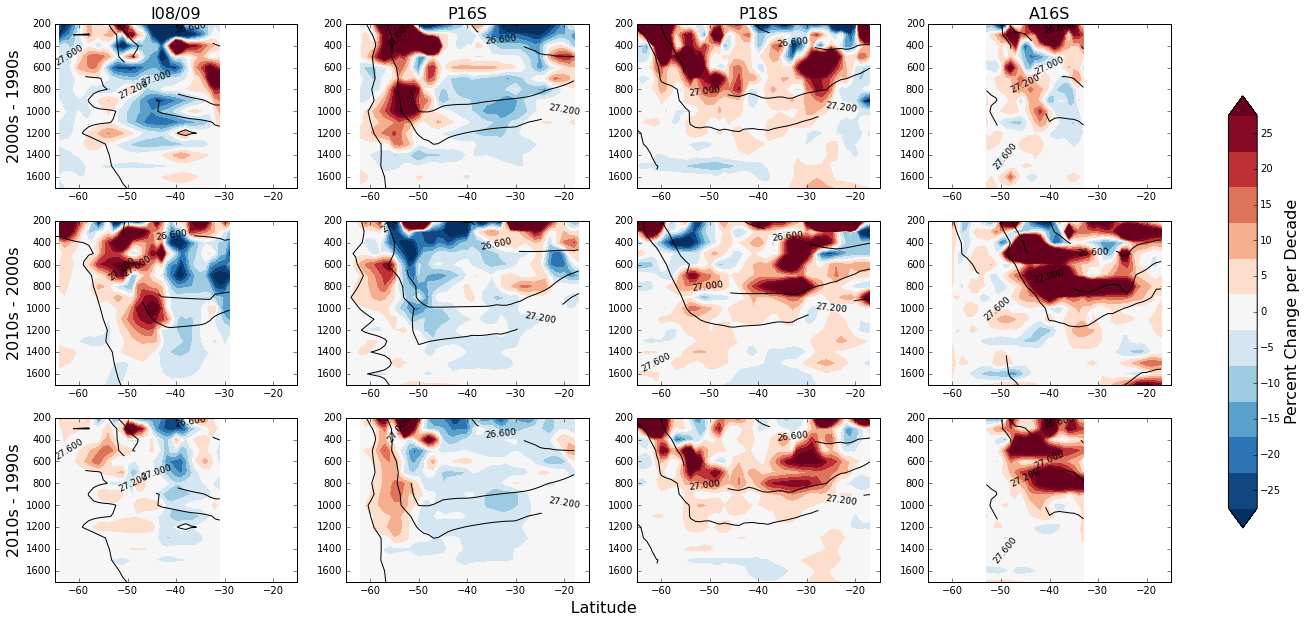
\includegraphics[height=3in]{AOU_change.png}
    \caption{Percent change per decade for AOU. }
\end{figure*}


















\end{document}
